\documentclass[12pt, a4paper, openany, oneside, titlepage]{book}	%opzione "twoside" anziché "oneside" per la stampa fronte-retro, "openrigth" anziché "openany" per far apparire i capitoli sempre a destra

\usepackage[italian]{babel}
\usepackage{fontenc}
\usepackage[tc]{titlepic}									%gestisce l'immagine nel frontespizio
%\usepackage[T1]{fontenc}
\usepackage[utf8]{inputenc}
\usepackage{indentfirst}									%indenta le prime righe
%\usepackage{emptypage}								%elimina la numerazione delle pagine bianche
\usepackage{fancyhdr}									%gestisce note a margine, note a piè di pagina, e intestazioni
\usepackage[pagebackref]{hyperref}						%gestisce i collegamenti ipertestuali
\usepackage[scaled=0.95]{helvet}\selectfont					%utilizza il font selezionato per tutto il documento
\usepackage{graphicx}									%include le figure
\usepackage{float}										%package per il posizionamento delle figure
\usepackage{amsmath}									%include l'ambiente matematico
\usepackage{enumitem}									%include l'ambiente per le enumerazioni
\usepackage{varwidth}									%permette di centrare le enumerazioni
\usepackage[nottoc]{tocbibind}							%gestisce il sommario
\usepackage{enumitem}									%permette di riprendere il conto di una enumerazione dove era stato interrotto
%\usepackage{clrscode3e}									%permette di scrivere pseudocodice (il file relativo si trova nella stessa cartella di questo sorgente Latex)
\usepackage{subfigure}									%permette di inserire sottofigure
\usepackage{amsfonts}									%gestisce il font matematico
\usepackage{amssymb}									%gestisce i simboli matematici
%\usepackage{epigraph}									%per la scrittura delle epigrafi a inizio capitolo
%\usepackage{midpage}									%per scrivere al centro della pagina
%\usepackage{extsizes}									%per utilizzare il tipo 'extbook'
\usepackage{listings}									%per inserire codice sorgente nel documento
\usepackage{color}										%per la gestione dei colori
\usepackage{pifont}									%introduce alcuni simboli
\usepackage{moresize}									%introduce nuove dimensioni per il testo
\usepackage{pdfpages}
\usepackage{rotating}

\pagestyle{fancy}
%\fancyhf{\small\thepage}
\fancyhead[RO, LE]{}										%solo i titotli dei capitoli in alto
%\fancyhead[RO, LE]{\small\thepage}
%\fancyhead[RE]{\small\nouppercase{\leftmark}}
%\fancyhead[RO,LE]{\small\thepage}

\def \openquote{``}										%alias per aprire le virgolette
\def \closequote{''}										%alias per chiudere le virgolette

\def \abs#1{\lvert #1 \rvert}								%alias per il simbolo di valore assoluto
\def \quote#1{\openquote #1\closequote}						%alias per il testo "virgolettato"

\newcommand{\accg}{\`}									%per i caratteri con accento grave
\newcommand{\acca}{\'}									%per i caratteri con accento acuto

\begin{document}
	\begin{titlepage}
		
		\title{Progetto di \vspace{2mm} \\ Sicurezza Informatica e Internet \\ \vspace{2 mm} {\large \bf{Progetto A2 - Encrypted 2D Barcodes}}}
		\author{Giovanni Rossi - \url{gio.rossi.1991@gmail.com}\\Pasquale Verlotta - \url{pasquale.verlotta@gmail.com} }
		\date{}%\today}
		\titlepic{
\includegraphics[width=5cm]{Immagini/logo_tor_vergata}}

	\end{titlepage}

	\maketitle

	\frontmatter

	\small

	\pagenumbering{Roman}

	\phantomsection

	\addcontentsline{toc}{chapter}{Indice}
	%\addcontentsline{toc}{chapter}{\listfigurename}

	\tableofcontents 
	\label{Indice}
	
	\listoffigures
	%\label{Elenco delle figure}

	%\listoftables

	\normalsize

	\mainmatter

	\def \ti{\textit}
\def \bf{\textbf}

\chapter{Introduzione}
	\label{cap:intro}
	
\section{Scopo del progetto}
	\label{sec:scopo}

Il progetto sviluppato in questi mesi per il corso di ``Sicurezza Informatica e Internet'' si propone come scopo quello di realizzare un'applicazione che permetta a due o più utenti di scambiarsi documenti cartacei in modo sicuro. In particolare questo significa che l'utente che utilizza tale sistema deve essere in grado di compilare un foglio con informazioni sensibili e di mandarlo ad un insieme di utenti facendo in modo che nessun altro al di fuori dei destinatari possa leggerne il contenuto. Viceversa i destinatari devono essere altrettanto sicuri del fatto che durante il trasferimento nessuno possa alterare il documento senza che chi lo riceve se ne accorga.
Quindi, riassumendo, il sistema dovrebbe permettere di:
\begin{itemize}
	\item compilare un documento contenente qualsiasi tipo di informazione;
	\item cifrare in tutto o in parte il documento appena scritto;
	\item allegare le informazioni cifrate al documento stesso così che il o i destinatari possano leggerlo;
	\item firmare il documento in modo tale che il mittente non possa ripudiarne la provenienza e i destinatari possano accorgersi di eventuali manomissioni durante il trasferimento;
	\item specificare diversi livelli di privilegio gerarchici per la lettura delle informazioni.
\end{itemize}
Quest'ultimo punto in particolare rappresenta un requisito importante. Può capitare, infatti, soprattutto in ambienti amministrativi, di voler pubblicare un certo documento pur mantenendo segrete alcune informazioni sensibili. In questo caso la soluzione più ovvia potrebbe essere quella di pubblicare versioni diverse dello stesso documento oscurando opportunamente sulle diverse copie le informazioni che si vogliono tenere segrete a ciascun gruppo. Questo processo può risultare lungo, macchinoso e poco sicuro: è possibile, infatti, che qualche copia possa finire al destinatario sbagliato se non si prendono precauzioni.

\section{Stato dell'arte}
	\label{sec:statoarte}

\section{Tecnologie Utilizzate}
	\label{sec:tecnologie}
	\def \ti{\textit}
\def \bf{\textbf}

\chapter{Progettazione}
	\label{cap:progettazione}
	
    In questo capitolo verranno analizzate in dettaglio le scelte progettuali che hanno permesso la realizzazione del sistema software, considerando le limitazioni riscontrate nell'architettura del sistema stesso. Dopodiché si analizzerà, attraverso la rappresentazione dei diagrammi \textbf{UML}, la definizione delle fasi di sviluppo, ossia la progettazione delle funzionalità correnti dell'applicazione.

\section{Requisiti}
	\label{sec:requisiti}
	Come primo aspetto della progettazione si analizzeranno adesso i requisiti del sistema. Innanzitutto si deve specificare che l'intero sistema è pensato per essere utilizzato in un ambito amministrativo dove gli utenti possono essere per esempio i dipendenti di un'azienda. Questo vuol dire che ci si trova in un sistema chiuso in cui le persone che usano il sistema sono note. Tuttavia è possibile che nel tempo i dipendenti si licenzino oppure che ne sopraggiungano di nuovi, quindi deve essere presente una procedura che consenta di inserire nuovi utenti ed eventualmente di rimuovere quelli esistenti. In questo sistema dove gli utenti sono noti, immaginiamo la presenza di un utente \textbf{amministratore} che agisce come supervisore ed è l'unico ad avere la facoltà di abilitare gli utenti all'utilizzo del servizio nonché di assegnare il \emph{Trust~Level}.

Di seguito viene mostrato il diagramma dei casi d'uso che rappresenta una vista generale delle funzionalità del sistema.
	\begin{center}	
		\begin{figure}[H]
		\centering
		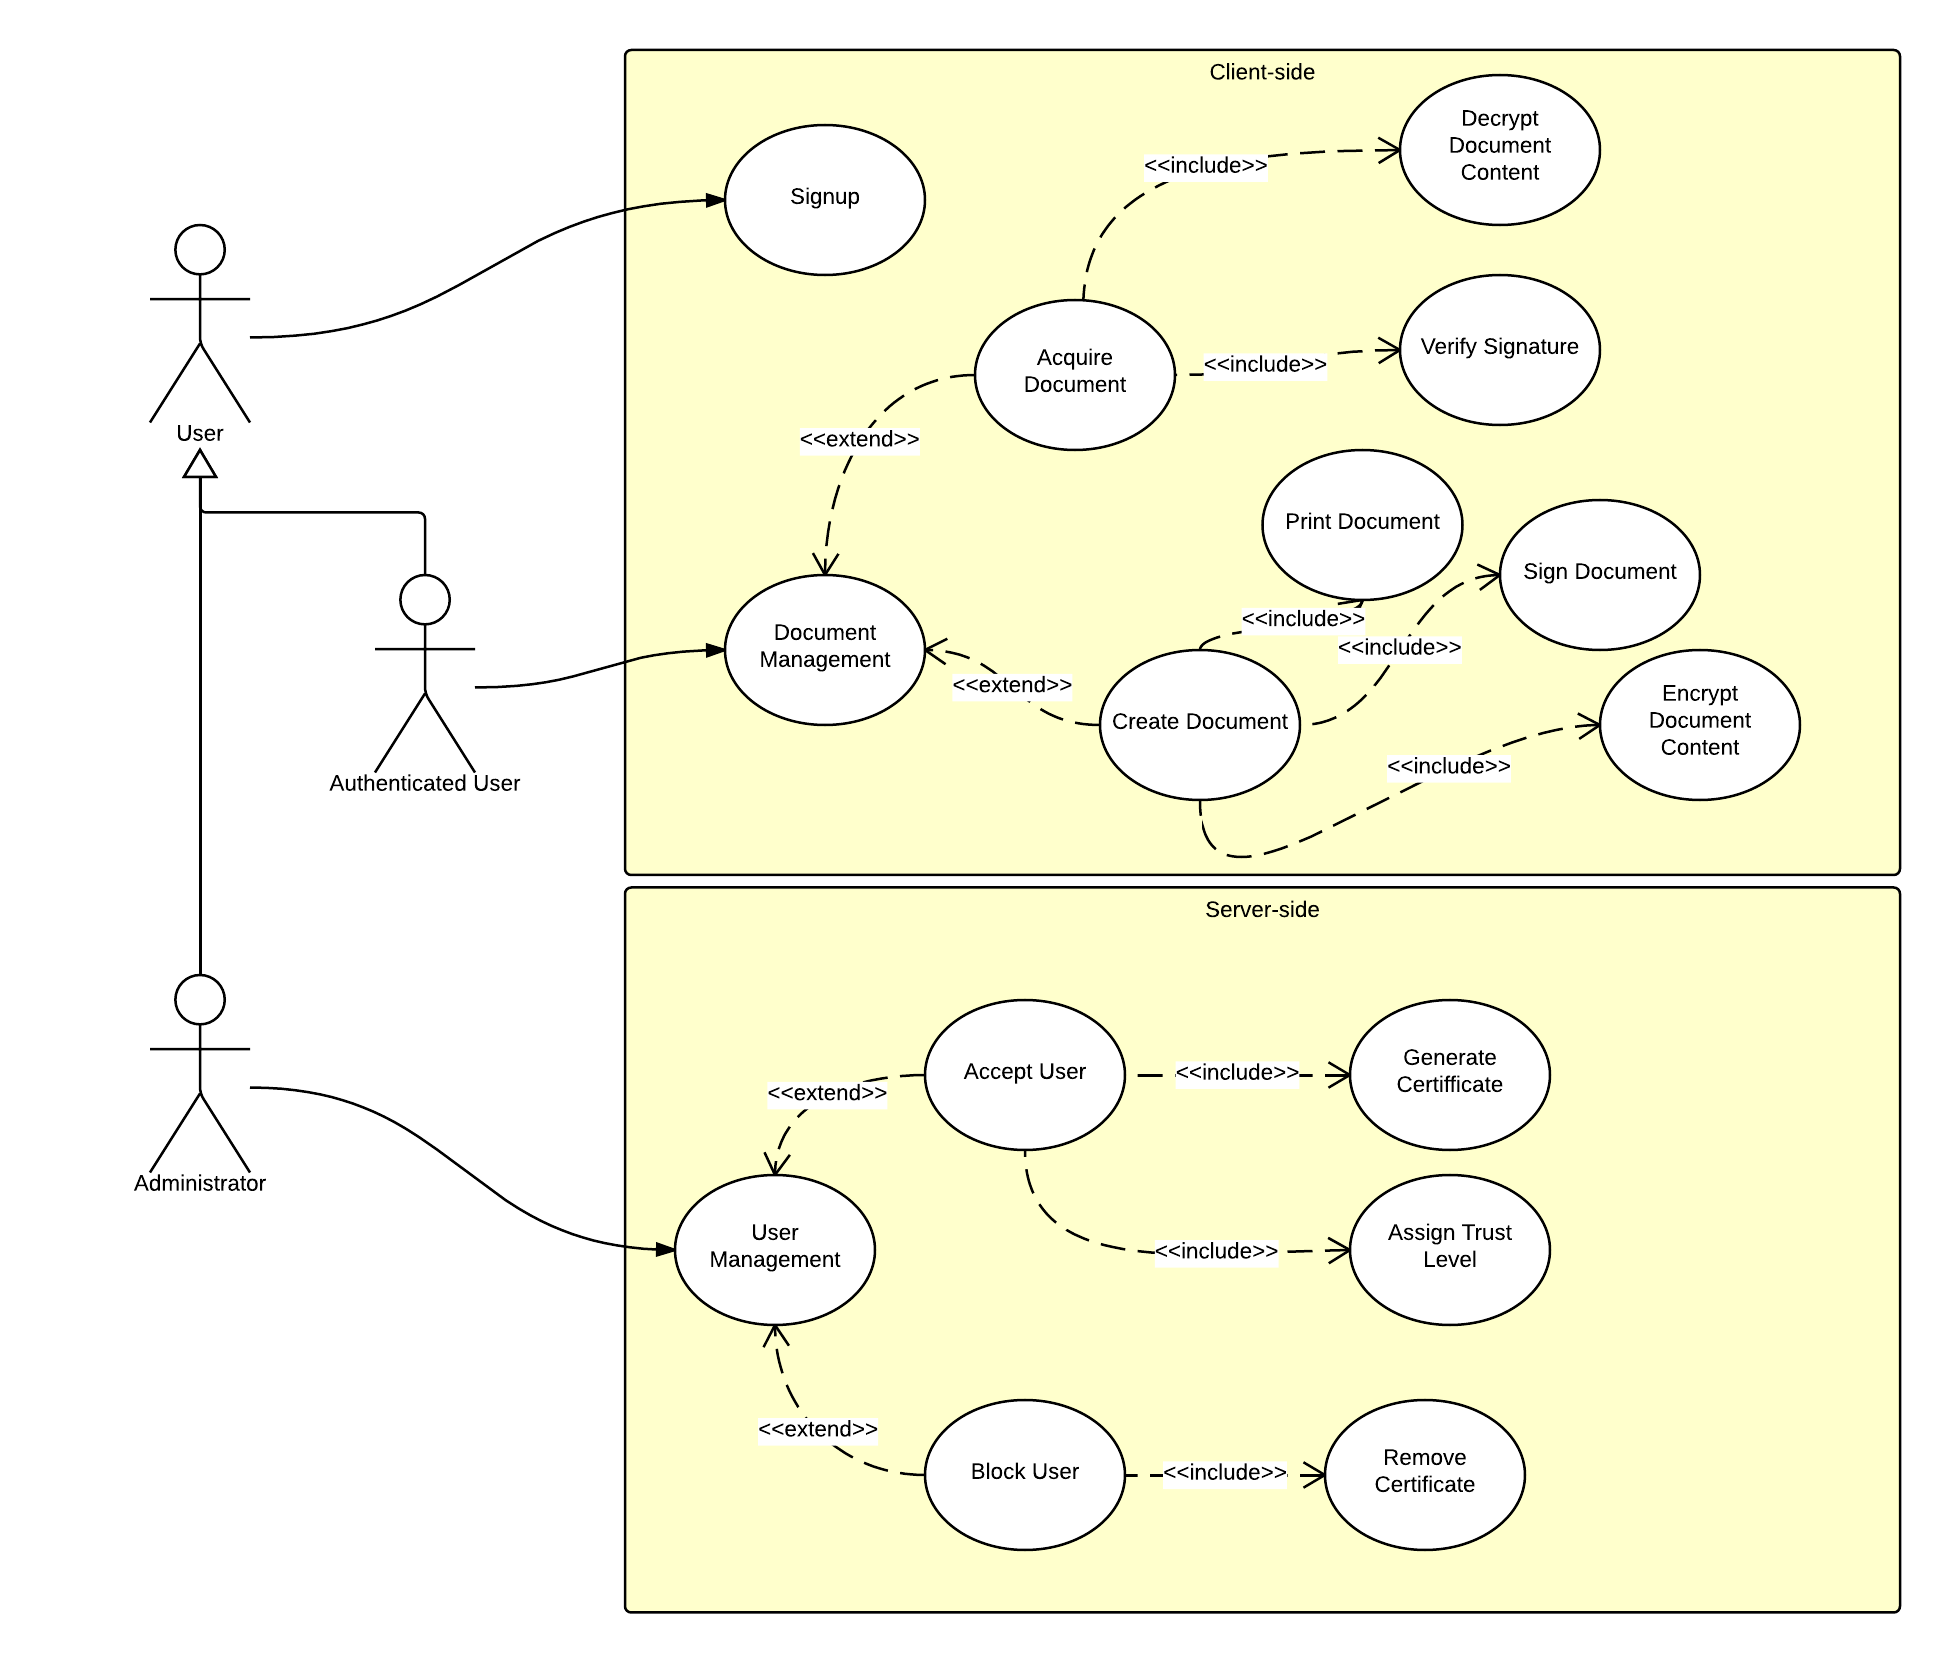
\includegraphics[scale=0.9]{Immagini/usecase}
		\caption[Use Case Diagram]{Diagramma dei casi d'uso del sistema software realizzato}
		\label{fig:usecase}
		\end{figure}
	\end{center}
La prima cosa che va evidenziata è che il tutto è strutturato secondo un architettura di tipo client/server. Questi due componenti dialogano tra di loro utilizzando una connessione sicura basata su SSL\footnote{Dettagli maggiori saranno dati nel paragrafo~\ref{sec:sicurezza}.}. Da quello che si può evincere, il server è un componente fondamentale che espone la funzionalità di \emph{provisioning} delle chiavi. Esso mantiene sia le chiavi di livello necessarie per la cifratura del documento, sia le chiavi pubbliche degli utenti registrati al sistema.

Da quello che si può vedere dalla figura~\ref{fig:usecase} nel sistema si hanno 3 attori importanti: l'amministratore, l'utente registrato (autenticato) e l'utente semplice che non ha mai utilizzato il sistema.
Come è stato già detto, l'amministratore si occupa di gestire l'accesso degli utenti. Questo vuol dire che ha piena facoltà di abilitare gli utenti all'utilizzo del sistema verificandone l'identità con procedure interne all'azienda che possono variare di caso in caso e che esulano completamente dagli scopi di questo progetto.
Oltre a questo può decidere di limitare l'accesso al sistema bloccando l'utente con una semplice procedura, grazie alla quale il server è in grado di comprendere se l'utente che si connette è autorizzato oppure no ad ottenere le chiavi di un certo livello.
Altro compito fondamentale è quello dell'assegnazione del Trust~Level che viene deciso in fase di abilitazione dell'utente al sistema. Tuttavia questo può essere anche cambiato successivamente. Grazie al Trust~Level, l'utente sarà abilitato a conoscere solo i segreti per cui è stato autorizzato, quindi l'assegnazione di questo parametro è fondamentale e richiede la massima attenzione.

L'utente registrato (o come riportato in figura~\ref{fig:usecase} ``autenticato'') rappresenta una qualsiasi persona che è stata abilitata dall'amministratore ad usare l'applicazione in tutte le sue funzionalità attuali. Un utente di questo tipo dispone di una coppia di chiavi asimmetriche RSA a $1024$ \texttt{bit} e di un certificato \texttt{X.509} che viene utilizzato per le connessioni al server che richiedono mutua autenticazione. L'utente autenticato ha la possibilità di comporre un documento, oscurarlo in alcune sue parti utilizzando le chiavi di livello a cui può accedere, e firmarlo con la propria chiave privata RSA. 
Naturalmente oltre alla composizione del documento, l'utente registrato ha anche la facoltà di leggere quello che è stato inviato a lui o agli utenti con il suo stesso Trust~Level\footnote{Si rimanda al paragrafo~\ref{sec:sicurezza} per una trattazione più approfondita di questo aspetto.}.

Per quanto riguarda l'utente semplice, si è sicuramente notato che questo ha l'unica facoltà di registrarsi al sistema. Questo perché non dispone ancora di un certificato da usare per l'autenticazione e quindi non ha alcuna possibilità di leggere le informazioni se non provando a fare un attacco sulla sicurezza del sistema o del documento cartaceo.

\section{Architettura}
	\label{sec:architettura}
Data una panoramica dei requisiti e delle funzionalità principali del sistema, si passerà adesso ad analizzare più in dettaglio l'architettura del sistema realizzato.
	\begin{center}	
		\begin{figure}[H]
		\centering
		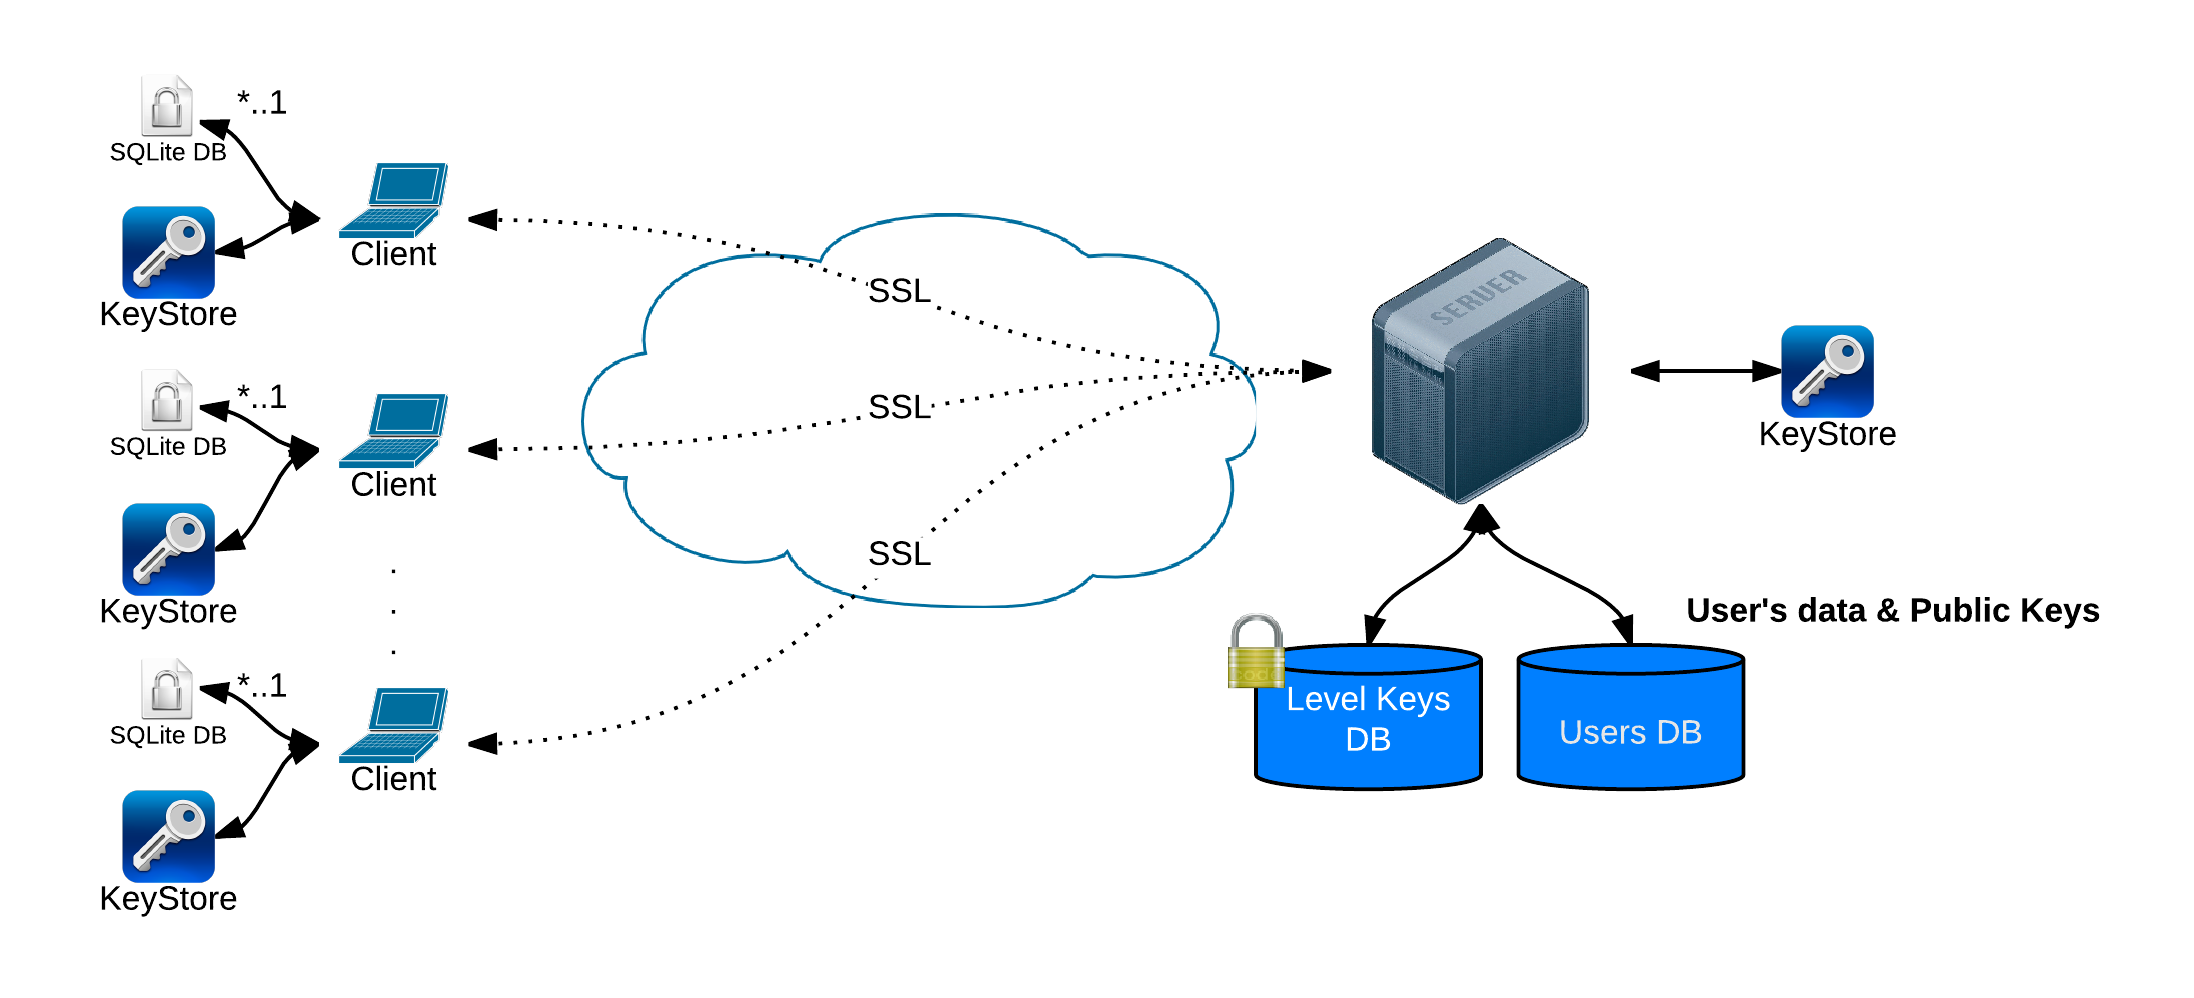
\includegraphics[scale=0.9]{Immagini/architettura}
		\caption[Architettura del sistema]{Questa figura rappresenta l'architettura del sistema software realizzato}
		\label{fig:usecase}
		\end{figure}
	\end{center}



\section{Gestione della sicurezza}
	\label{sec:sicurezza}
	%login - autenticazione forte
	%come si cripta: singolo/molti utenti
	%come si descripta
	%connessione al server
	%connessioni SSL - gestione certificati/keystore/mutua autenticazione	
	\chapter{Funzionamento dell'applicazione}
	\label{cap:funzionamento}		
In questo capitolo si illustreranno le modalità di funzionamento dell'applicazione implementata.
Come già detto nel capitolo~\ref{cap:progettazione}, l'applicazione si compone di due parti: server e client.

\section{Server}

Il server ha lo scopo di gestire gli utenti, i certificati relativi e di distribuire le chiavi di livello e le chiavi pubbliche degli utenti certificati.

L'applicativo può essere eseguito in due modi:
\begin{itemize}
	\item da riga di comando tramite l'istruzione:\\ \texttt{java -jar -DprogettoSII.configuration=<path-to-conf.properties> <path-to-jar>/server.jar};
	\item tramite l'IDE \emph{Eclipse} impostando opportunamente il percorso del file \texttt{conf.properties} nella configurazione di esecuzione (\textbf{Run Configuration}).  
\end{itemize}

Se l'applicazione viene lanciata da riga di comando è necessario inserire una password che serve a sbloccare il keystore. Dopo aver eseguito questo passaggio è possibile impartire comandi al server direttamente dal terminale. I comandi che sono disponibili ora sono: \texttt{quit} e \texttt{adminconf}.
Il primo chiude il server in maniera \emph{graceful} mentre il secondo avvia l'interfaccia grafica che consente all'amministratore di interagire con i dati degli utenti.
	\begin{center}	
		\begin{figure}[H]
		\centering
		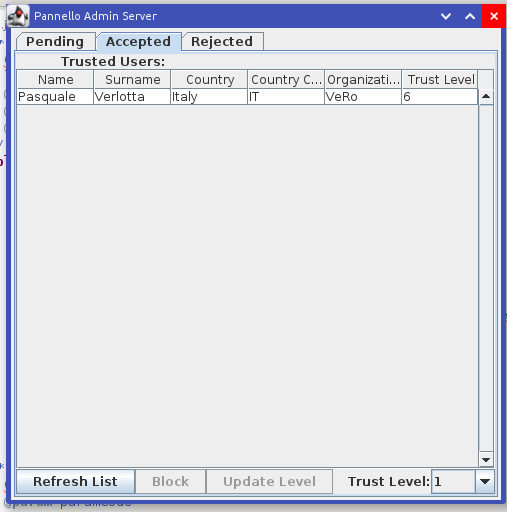
\includegraphics[scale=0.7]{Immagini/server_accepted}
		\caption[GUI del server]{Interfaccia grafica del server.}
		\label{fig:servergui}
		\end{figure}
	\end{center}
Come si vede nella figura~\ref{fig:servergui} ci sono tre schede riferite ad altrettante liste: 
\begin{itemize}
	\item \textbf{Pending} in cui compare la lista degli utenti che intendono registrarsi al sistema e attendono l'intervento dell'amministratore ;
	\item \textbf{Accepted} in cui c'è la lista degli utenti certificati che sono autorizzati all'accesso al sistema;
	\item \textbf{Rejected} in cui compare la lista degli utenti bloccati a cui è negato l'accesso.
\end{itemize}
I pulsanti in basso consentono di accettare o rifiutare o aggiornare le richieste degli utenti.

\section{Client}
Il client ha lo scopo di gestire le funzionalità di registrazione, login, cifratura e decriptazione.
La registrazione consiste nel riempire un form con dati anagrafici e i percorsi dei file delle cartelle necessarie per salvare i documenti cifrati/decifrati. Se la registrazione va a buon fine, cioè il server autentica l'utente, viene rilasciato un \textbf{SecureID}, che insieme con i dati inseriti viene scritto su un pdf generato automaticamente e salvato nella cartella di output scelta.
Il login consente di accedere all'applicazione e consiste nel riempire un form con Nome, Cognome, Password e il Codice rilasciato all'atto della registrazione. 

	\begin{center}	
		\begin{figure}[H]
		\centering
		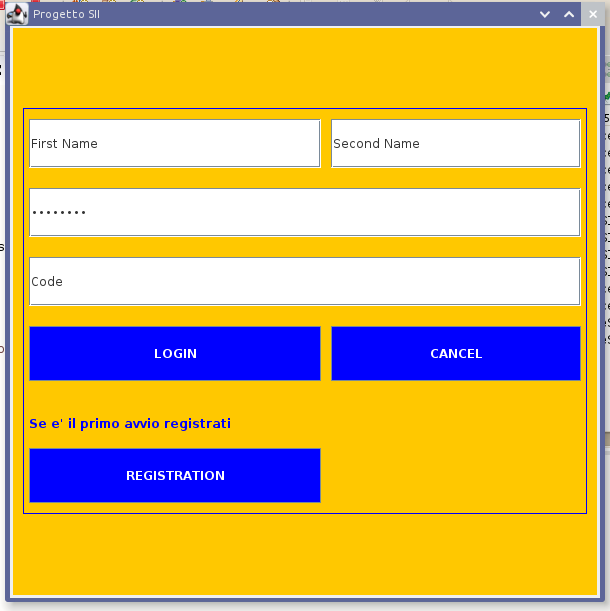
\includegraphics[scale=0.7]{Immagini/login}
		\caption[Login]{GUI di login}
		\label{fig:login}
		\end{figure}
	\end{center}
	
Dopo aver effettuato il login si accede alla schermata principale

	\begin{center}	
		\begin{figure}[H]
		\centering
		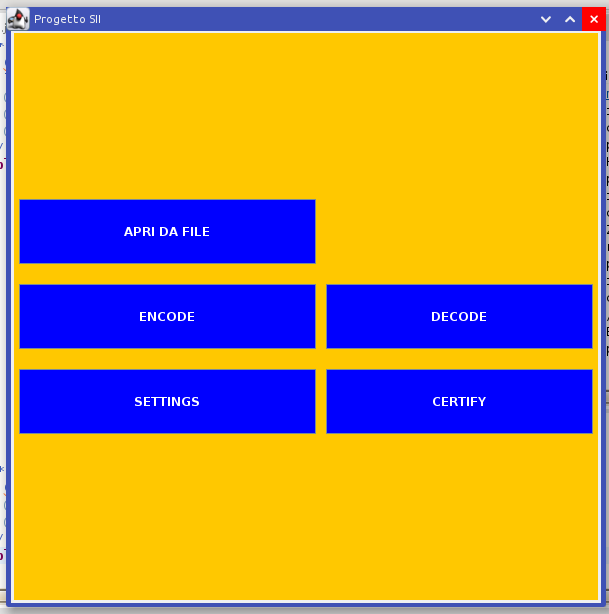
\includegraphics[scale=0.7]{Immagini/homelayout}
		\caption[homelayout]{GUI della schermata principale}
		\label{fig:home}
		\end{figure}
	\end{center}
	
Da questa schermata si accede alle funzionalità dell'applicazione cliccando i diversi pulsanti
\begin{itemize}
	\item \textbf{APRI} - consente di scegliere un file dal file system locale. Se il file scelto è un'immagine viene caricata la GUI per la decodifica, mentre se il file è un testo (.txt) viene caricata la GUI per la codifica;
	\item \textbf{ENCODE} - carica la GUI per la codifica;
	\item \textbf{DECODE} - carica la GUI per la decodifica;
	\item \textbf{CERTIFY} - la funzionalità necessaria per essere abilitati alla codifica e decodifica. Al primo login occorre, infatti, scaricare il certificato dal server, se l'amministratore ha autorizzato l'utente, ed aggiornarne i dati. 
\end{itemize}

\subsection{Cifratura}
La seguente figura~\ref{fig:encode} illustra la GUI per la composizione di un file da criptare. Vi si accede cliccando \textbf{ENCODE} nella schermata principale, e selezionando un file.

	\begin{center}	
		\begin{figure}[H]
		\centering
		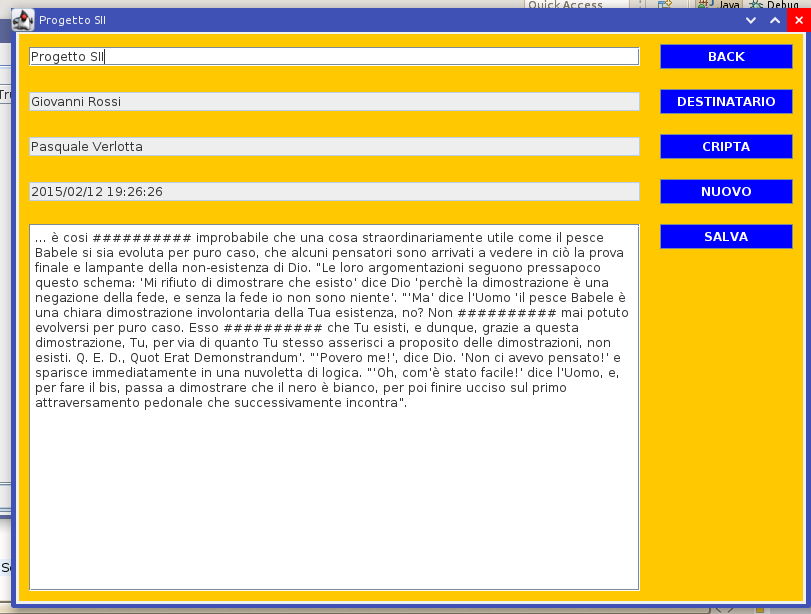
\includegraphics[scale=0.6]{Immagini/writelayout}
		\caption[GUI di encode]{Intefaccia grafica per la codifica}
		\label{fig:encode}
		\end{figure}
	\end{center}
	
La schermata si compone di cinque campi:
\begin{itemize}
	\item Il \textbf{titolo}  che comparirà nell'intestazione del documento;
	\item L'\textbf{autore} del documento, che viene riempito in automatico con il nome e cognome dell'utente loggato;
	\item Il \textbf{destinatario} che viene impostato tramite il pulsante \textbf{DESTINATARIO}, che consente di scegliere se cifrare per un singolo utente, o per un livello;
	\item Le \textbf{informazioni} che per il momento consistono in data e ora della creazione del documento;
	\item L'area nella quale verrà inserito automaticamente il testo preso dal file selezionato.
\end{itemize}
e di cinque pulsanti, con funzioni autoesplicative. 

Una volta selezionato il destinatario del documento si seleziona il testo da cifrare e si preme il pulsante \textbf{CRIPTA} che esegue la cifratura tramite RSA con la chiave pubblica del destinatario o tramite AES con le chiavi di livello, partendo dal livello 1 fino al livello scelto, ed infine sostituisce il testo selezionato con una serie di hashtag.
Il pulsante \textbf{SALVA} genera il QR-Code contente la firma del documento cifrata, il QR-Code con le informazioni in chiaro per decriptare, e i QR-Code relativi alle parti di testo criptate. Una volta terminata la cifratura viene generata l'immagine come descritto nel capitolo \ref{cap:progettazione}.

\subsection{Decifrazione}
La seguente figura~\ref{fig:decode} illustra la GUI per la composizione di un file da decriptare. Vi si accede cliccando \textbf{DECODE} nella schermata principale, e selezionando un file.
	
	\begin{center}	
		\begin{figure}[H]
		\centering
		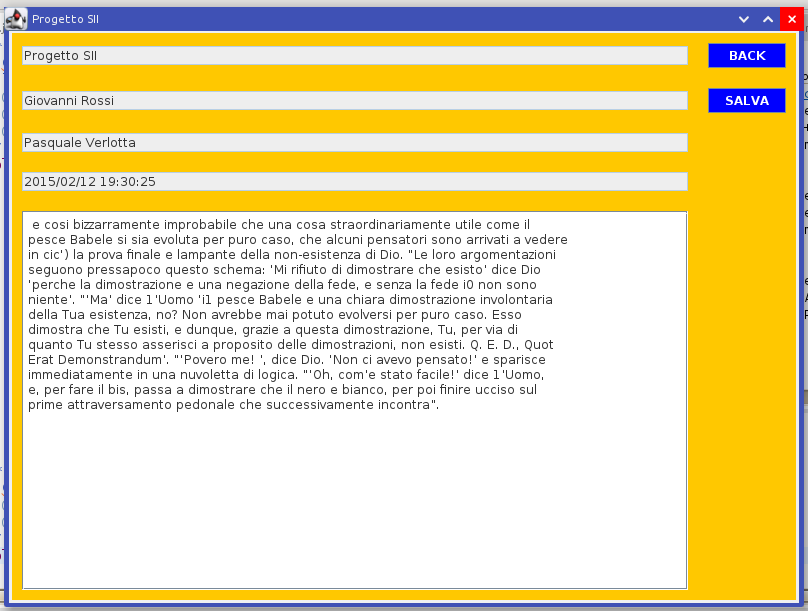
\includegraphics[scale=0.6]{Immagini/readlayout}
		\caption[GUI di decode]{Interfaccia grafica per la decodifica}
		\label{fig:decode}
		\end{figure}
	\end{center}

La GUI ha gli stessi campi della GUI per l'encode, con la differenza che questi sono riempiti in automatico dal sistema in fase di decriptazione del documento e il testo è in chiaro, decriptato quindi.
Nel caso il testo contenga ancora gli hashtag significa che non si ha il privilegio di decriptare il file, perché o non si ha il livello autoritativo necessario o non si è il destinatario del documento.
	\def \ti{\textit}
\def \bf{\textbf}

\chapter{Conclusioni}
		\label{cap:conclusioni}

	%\appendix

\end{document}